\chapter{Исследовательская часть}

В данном разделе будут приведены примеры работы программы, а также проведен сравнительный анализ алгоритмов при различных ситуациях на основе полученных данных.

\section{Технические характеристики}

Технические характеристики устройства, на котором выполнялось тестирование представлены далее:
\begin{itemize}[label={---}]
	\item операционная система: Windows 11, x64;
	\item оперативная память: 8 Гб;
	\item процессор: AMD Ryzen 5 5500U с видеокартой Radeon Graphics 2.10~ГГц.
\end{itemize}

Во время замеров времени ноутбук был нагружен только встроенными приложениями окружения.

\section{Демонстрация работы программы}

На рисунке~\ref{img:run} представлен результат работы программы.

\begin{figure}[H]
	\center{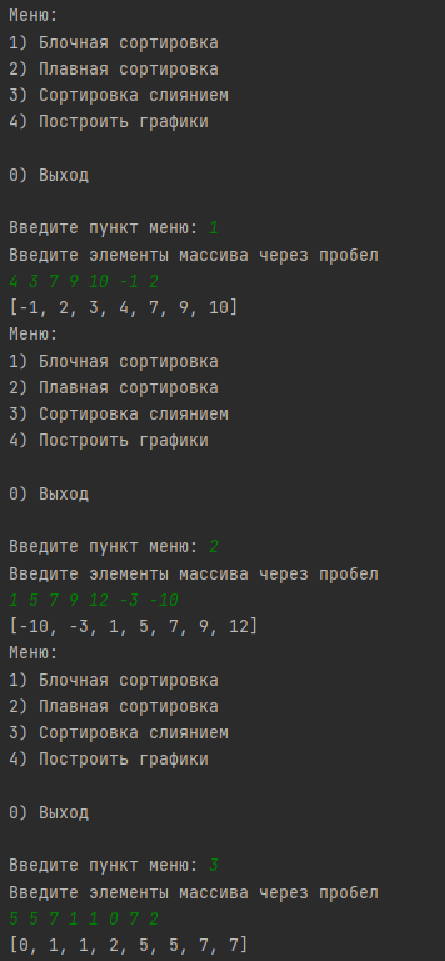
\includegraphics[scale=1.5]{img/run}}
	\caption{Пример работы программы}
	\label{img:run}
\end{figure}
\clearpage

\section{Время выполнения алгоритмов}

Как было сказано выше, используется функция замера процессорного времени process\_time из библиотеки time на Python. Функция возвращает пользовательское процессорное время типа float.

Использовать функцию приходится дважды, затем из конечного времени нужно вычесть начальное, чтобы получить результат.

Замеры проводились для размеров массива от 100 до 500 с шагом 50 по 5000 раз на различных входных данных.

Результаты замеров приведены в таблицах~\ref{tbl:time_mes_rand}---~\ref{tbl:time_mes_rev} (время в мс).

\begin{table}[H]
	\begin{center}
		\begin{threeparttable}
			\captionsetup{justification=raggedright, singlelinecheck=off}
			\caption{Результаты замеров времени для произвольных массивов}
			\label{tbl:time_mes_rand}
			\begin{tabular}{|c|c|c|c|}
				\hline
				Размер массива & Блочная сорт., мс & Плавная сорт., мс & Сорт. слиянием, мс\\
				\hline
				100&0.263&0.075&0.163\\
				\hline
				150&0.428&0.097&0.278\\
				\hline
				200&0.603&0.150&0.375\\
				\hline
				250&0.803&0.119&0.528\\
				\hline
				300&0.922&0.106&0.634\\
				\hline
				350&1.134&0.188&0.722\\
				\hline
				400&1.297&0.200&0.825\\
				\hline
				450&1.422&0.216&0.925\\
				\hline
				500&1.647&0.256&1.084\\
				\hline
			\end{tabular}
		\end{threeparttable}
	\end{center}
\end{table}

\begin{table}[H]
	\begin{center}
		\begin{threeparttable}
			\captionsetup{justification=raggedright, singlelinecheck=off}
			\caption{Результаты замеров времени для отсортированных массивов}
			\label{tbl:time_mes_sort}
			\begin{tabular}{|c|c|c|c|}
				\hline
				Размер массива & Блочная сорт., мс & Плавная сорт., мс & Сорт. слиянием, мс\\
				\hline
				100&0.166&0.066&0.241\\
				\hline
				150&0.256&0.081&0.400\\
				\hline
				200&0.334&0.109&0.559\\
				\hline
				250&0.375&0.144&0.744\\
				\hline
				300&0.509&0.178&1.019\\
				\hline
				350&0.625&0.197&1.078\\
				\hline
				400&0.731&0.178&1.194\\
				\hline
				450&0.912&0.234&1.325\\
				\hline
				500&0.981&0.231&1.641\\
				\hline
			\end{tabular}
		\end{threeparttable}
	\end{center}
\end{table}

\begin{table}[H]
	\begin{center}
		\begin{threeparttable}
			\captionsetup{justification=raggedright, singlelinecheck=off}
			\caption{Результаты замеров времени для отсортированных в обратном порядке массивов}
			\label{tbl:time_mes_rev}
			\begin{tabular}{|c|c|c|c|}
				\hline
				Размер массива & Блочная сорт., мс & Плавная сорт., мс & Сорт. слиянием, мс\\
				\hline
				100&0.150&0.081&0.269\\
				\hline
				150&0.241&0.109&0.416\\
				\hline
				200&0.369&0.122&0.613\\
				\hline
				250&0.403&0.144&0.681\\
				\hline
				300&0.491&0.119&0.950\\
				\hline
				350&0.616&0.188&1.019\\
				\hline
				400&0.756&0.216&1.234\\
				\hline
				450&0.769&0.203&1.359\\
				\hline
				500&0.909&0.212&1.616\\
				\hline
			\end{tabular}
		\end{threeparttable}
	\end{center}
\end{table}


На рисунках~\ref{img:graphrand}---~\ref{img:graphworst} приведена визуализация результатов замеров.

\inputPdf{graphrand}{Визуализация результатов замеров для произвольных массивов}

\inputPdf{graphbest}{Визуализация результатов замеров для отсортированных массивов}

\inputPdf{graphworst}{Визуализация результатов замеров для отсортированных в обратном порядке массивов}

\section{Вывод}

В результате эксперимента было получено, что наиболее эффективной по времени является реализация плавной сортировки. Она дает преимущество при любых входных данных: произвольных, отсортированных, отсортированных в обратном порядке. Например, при количестве элементов массива равном 500 реализация алгоритма плавной сортировки дает преимущество в 84\% перед реализацией алгоритма блочной сортировки и в 76\% перед реализацией алгоритма сортировки слиянием.